\section{Electrostatics}


\begin{Exercise}[difficulty=1]
Using Gauss law find a electric field $E$ in vicinity of point charge $Q$.
\end{Exercise}

\begin{Exercise}[difficulty=2]
Show that Coulomb's law can be derived from Gauss law.
\end{Exercise}

\begin{Exercise}[difficulty=2]
Find electric field $\vec{E}$ in point $P$, which is exactly in the middle between two point charges $Q_1$ and $Q_2$. 
%\begin{center}
%\includegraphics[scale=0.1]{test.pdf} 
%\end{center}
\end{Exercise}

\begin{Exercise}[difficulty=3]
Using Gauss's Law find formula describing electric field intensity E on the line between two charges ($Q_1$,$Q_2$). 
\begin{center}
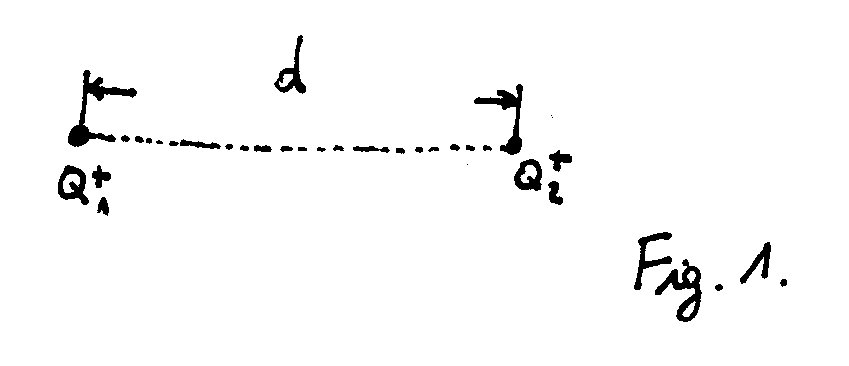
\includegraphics[scale=0.3]{img/fig_e1.png} 
\end{center}
\end{Exercise}

\begin{Exercise}[difficulty=3]
What is the distribution of electric field inside and outside of the dielectric ball charged with uniform volume density $\rho$?
\begin{center}
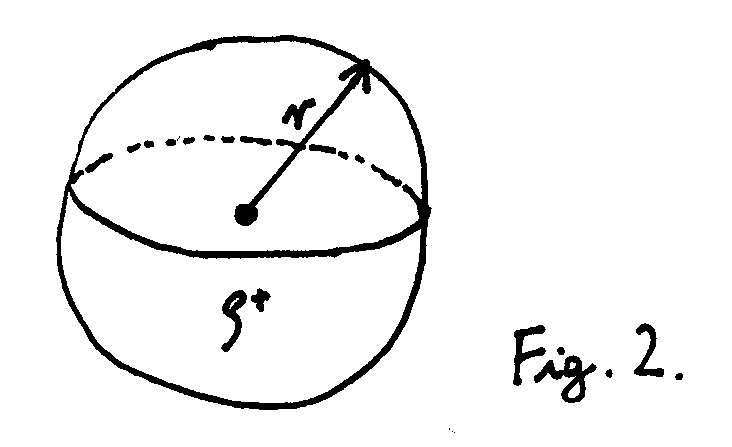
\includegraphics[scale=0.3]{img/fig_e2.png} 
\end{center}
\end{Exercise}

\begin{Exercise}[difficulty=4]
What is the distribution of electric field inside and outside of the dielectric ball with charge density given by function $\rho(r)= r^2$?
\end{Exercise}


\begin{Exercise}[difficulty=3]
Find the electric displacement field distribution in the vicinity of the plane charged with surface density $\rho_s$.
\begin{center}
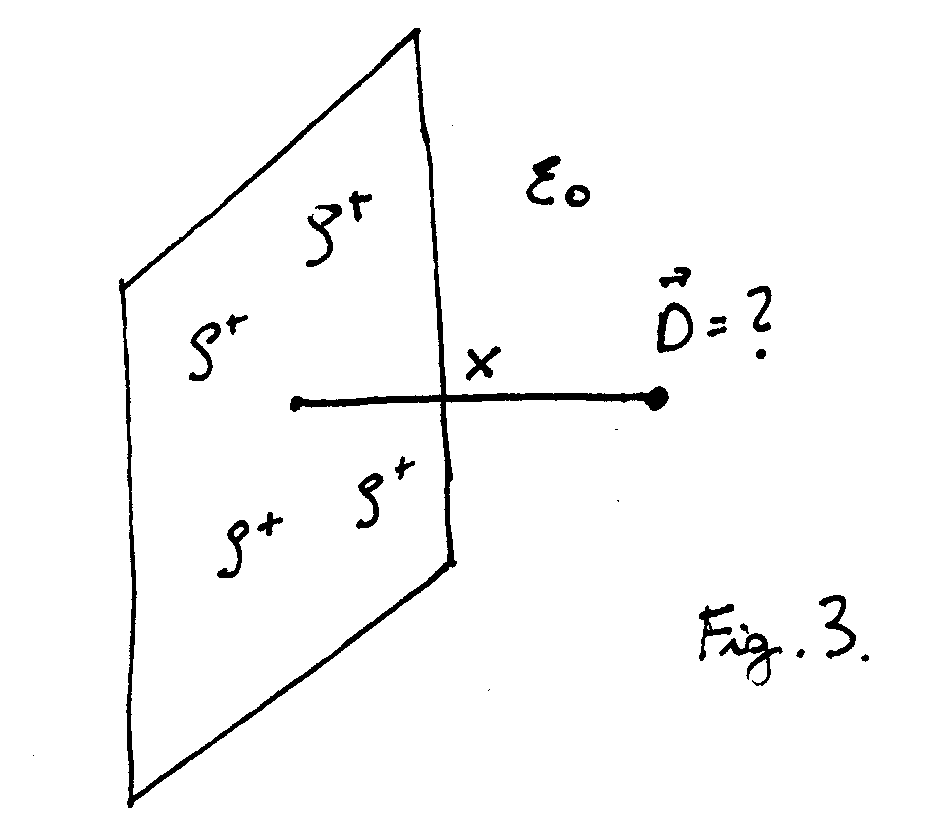
\includegraphics[scale=0.3]{img/fig_e3.png} 
\end{center}
\end{Exercise}

